%!TEX root = ../../WTG.tex

\begin{figure}
	\centering
	\subcaptionbox{Ausgangsnetzwerk}[0.49\textwidth]{
		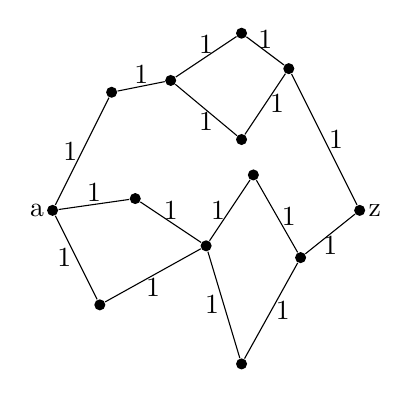
\begin{tikzpicture}[scale=1.5, every node/.style=fill,circle,minimum size=4pt,inner sep=0pt]
			\node [label=left:{a}] (a) at (0,0) {};
			\node (1) at (0.5,1) {};
			\node (2) at (1,1.1) {};
			\node (3) at (1.6,1.5) {};
			\node (4) at (1.6,0.6) {};
			\node (5) at (2,1.2) {};
			\node[label=right:{z}] (z) at (2.6,0) {}; 
			\node (6) at (0.7,0.1) {};
			\node (7) at (0.4,-0.8) {};
			\node (8) at (1.3,-0.3) {};
			\node (9) at (1.7,0.3) {};
			\node (10) at (1.6,-1.3) {};
			\node (11) at (2.1,-0.4) {};
			\draw (a) -- (1) node [midway, left, fill=none] {1};	
			\draw (1) -- (2) node [midway, above, fill=none] {1};	
			\draw (2) -- (3) node [midway, above, fill=none] {1};	
			\draw (2) -- (4) node [midway, below, fill=none] {1};
			\draw (4) -- (5) node [midway, right, fill=none] {1};		
			\draw (3) -- (5) node [midway, above, fill=none] {1};	
			\draw (5) -- (z) node [midway, right, fill=none] {1};	
			\draw (a) -- (6) node [midway, above, fill=none] {1};
			\draw (a) -- (7) node [midway, left, fill=none] {1};
			\draw (6) -- (8) node [midway, above, fill=none] {1};
			\draw (7) -- (8) node [midway, below, fill=none] {1};	
			\draw (8) -- (9) node [midway, left, fill=none] {1};	
			\draw (8) -- (10) node [midway, left, fill=none] {1};
			\draw (9) -- (11) node [midway, right, fill=none] {1};	
			\draw (10) -- (11) node [midway, right, fill=none] {1};	
			\draw (11) -- (z) node [midway, below, fill=none] {1};						
			%\draw (d) -- \node at (1,1) {} \node[fill=none,midway,label=above:{1}] {};
		\end{tikzpicture}
	}
	\hfill
	\subcaptionbox{Reihenschaltungen zusammengezogen}[0.49\textwidth]{
		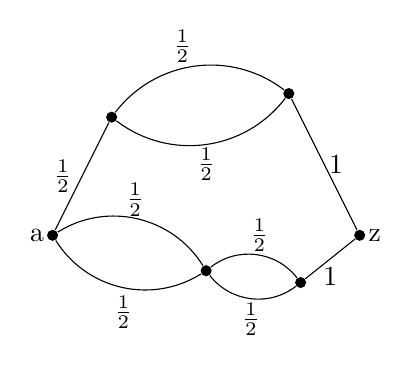
\begin{tikzpicture}[scale=1.5, every node/.style=fill,circle,minimum size=4pt,inner sep=0pt]
		\node [label=left:{a}] (a) at (0,0) {};
		\node (1) at (0.5,1) {};
		\node (2) at (2,1.2) {};
		\node[label=right:{z}] (z) at (2.6,0) {}; 
		\node (3) at (1.3,-0.3) {};
		\node (4) at (2.1,-0.4) {};
		
		\draw (a) -- (1) node [midway, left, fill=none] {$\frac{1}{2}$};
		\draw[bend angle=45,bend left] (1) to (2);
		\node [fill=none] at (1.1,1.6) {$\frac{1}{2}$};
		\draw[bend angle=45,bend right] (1) to (2);
		\node [fill=none] at(1.3,0.6) {$\frac{1}{2}$};
		\draw (2) -- (z) node [midway, right, fill=none] {$1$};
		\draw[bend angle=45,bend left] (a) to (3);
		\node [fill=none] at (0.7,0.3){$\frac{1}{2}$};
		\draw[bend angle=45,bend right] (a) to (3);
		\node [fill=none] at(0.6,-0.65) {$\frac{1}{2}$};	
		\draw[bend angle=45,bend left] (3) to (4);
		\node [fill=none] at (1.75,0) {$\frac{1}{2}$};
		\draw[bend angle=45,bend right] (3) to (4);
		\node [fill=none] at (1.68,-0.71) {$\frac{1}{2}$};	
		\draw (4) -- (z) node [midway, below=2pt, fill=none] {$1$};				
		%\draw (d) -- \node at (1,1) {} \node[fill=none,midway,label=above:{1}] {};
		\end{tikzpicture}
	}
	\hfill
	\subcaptionbox{Parallelschaltungen zusammengezogen}[0.30\textwidth]{
		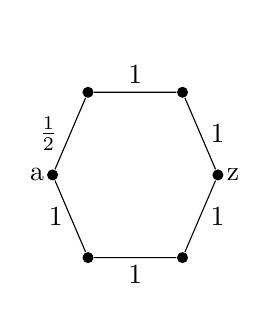
\begin{tikzpicture}[scale=1.5, every node/.style=fill,circle,minimum size=4pt,inner sep=0pt]
			\node [label=left:{a}] (a) at (0,0) {};
			\node (1) at (0.3,0.7) {};
			\node (2) at (1.1,0.7) {};
			\node[label=right:{z}] (z) at (1.4,0) {}; 
			\node (3) at (0.3,-0.7) {};
			\node (4) at (1.1,-0.7) {};
			\draw (a) -- (1) node [midway, left=1pt, fill=none] {$\frac{1}{2}$};
			\draw (1) -- (2) node [midway, above=2pt, fill=none] {$1$};
			\draw (2) -- (z) node [midway, right=2pt, fill=none] {$1$};
			\draw (a) -- (3) node [midway, left=1pt, fill=none] {$1$};
			\draw (3) -- (4) node [midway, below=2pt, fill=none] {$1$};
			\draw (4) -- (z) node [midway, right=2pt, fill=none] {$1$};
			\node[fill=none] at (0,-0.8) {}; 
			\node[fill=none] at (0,1.2) {};	
		\end{tikzpicture}
	}
	\hfill
	\subcaptionbox{Reihenschaltungen erneut zusammengezogen}[0.30\textwidth]{
		\begin{tikzpicture}[scale=1.5, every node/.style=fill,circle,minimum size=4pt,inner sep=0pt]
			\node [label=left:{a}] (a) at (0,0) {};
			\node[label=right:{z}] (z) at (1.4,0) {}; 
			\draw[bend angle=45,bend right] (a) to (z);
			\node [fill=none] at (0.7,0.5) {$\frac{1}{4}$};
			\draw[bend angle=45,bend left] (a) to (z);
			\node [fill=none] at (0.7,-0.5) {$\frac{1}{3}$};
			\node[fill=none] at (0,-0.8) {}; 
			\node[fill=none] at (0,1.2) {};
		\end{tikzpicture}
	}
	\hfill
	\subcaptionbox{Parallelschaltungen erneut zusammengezogen}[0.30\textwidth]{
		\begin{tikzpicture}[scale=1.5, every node/.style=fill,circle,minimum size=4pt,inner sep=0pt]
		\node [label=left:{a}] (a) at (0,0) {};
		\node[label=right:{z}] (z) at (1.4,0) {}; 
		\node[fill=none] at (0,-0.8) {}; 
		\node[fill=none] at (0,1.2) {};
		\draw (a) to (z);
		\node [fill=none] at (0.7,0.2) {$\frac{7}{12}$};
		\end{tikzpicture}	
	}
	\caption{Schritt für Schritt Simplifizierung eines Netzwerks}
	\label{fig:1-5}
\end{figure}